\section*{Question 6}
\fakesection{6}

This problem compares the performance of the Cooley-Tukey FFT algorithm to a naive DFT. Beginning with the DFT, for an input sequence $\{x_n\}$ of length $N$, the DFT computes:
\begin{align}
    X_k = \sum_{n=0}^{N-1} x_n \cdot e^{-\frac{i2\pi}{N}kn},\ k = 0 \ldots N - 1
\end{align}
Each of the $N$ summations has $N$ terms, giving a tight bound on the time complexity in $\Theta(N^2)$. Compare this to the general case of the Cooley-Tukey algorithm, visualised in Figure \ref{fig:viz_cooley_tukey}.

\begin{figure}[ht]
    \centering
    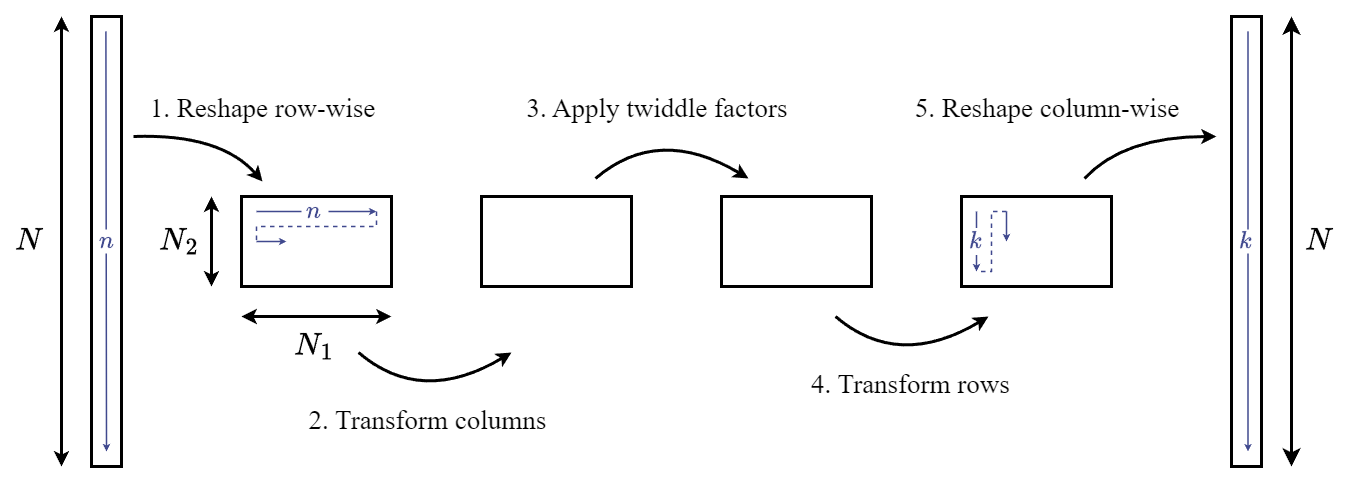
\includegraphics[width=0.9\textwidth]{images/q6_viz_cooley_tukey.png}
    \caption{Visualisation of the Cooley-Tukey algorithm (general case)}
    \label{fig:viz_cooley_tukey}
\end{figure}

In words, where $N_1N_2=N$, the algorithm:
\begin{enumerate}
    \item Reshapes the input into an $N_1\times N_2$ row-major matrix; time complexity in $\Theta(N)$.
    \item Performs DFT on each column; in $\Theta(N_1N_2^2)$.
    \item Applies twiddle factors to each element to rectify phase errors introduced by packing the signal into an aligned matrix; in $\Theta(N)$.
    \item Performs DFT on each row; in $\Theta(N_2N_1^2)$.
    \item Reshapes the matrix in column-major order back into a vector; in $\Theta(N)$.
\end{enumerate}
The overall time complexity is in:
\begin{align}
    \Theta(N_1N_2^2) + \Theta(N_2N_1^2) + \Theta(N) \subset \Theta(N(N_1+N_2))
\end{align}
Given $N_1+N_2<N_1N_2=N$, we have $\Theta(N(N_1+N_2))\subset \Theta(N^2)$ and so we conclude that the Cooley-Tukey FFT is asymptotically faster than the DFT. We test this on the 15-point signal of Figure \ref{fig:q6_signal}; the Fourier transform is also calculated using \texttt{scipy.fft} as a reference.

\begin{figure}[ht]
    \centering
    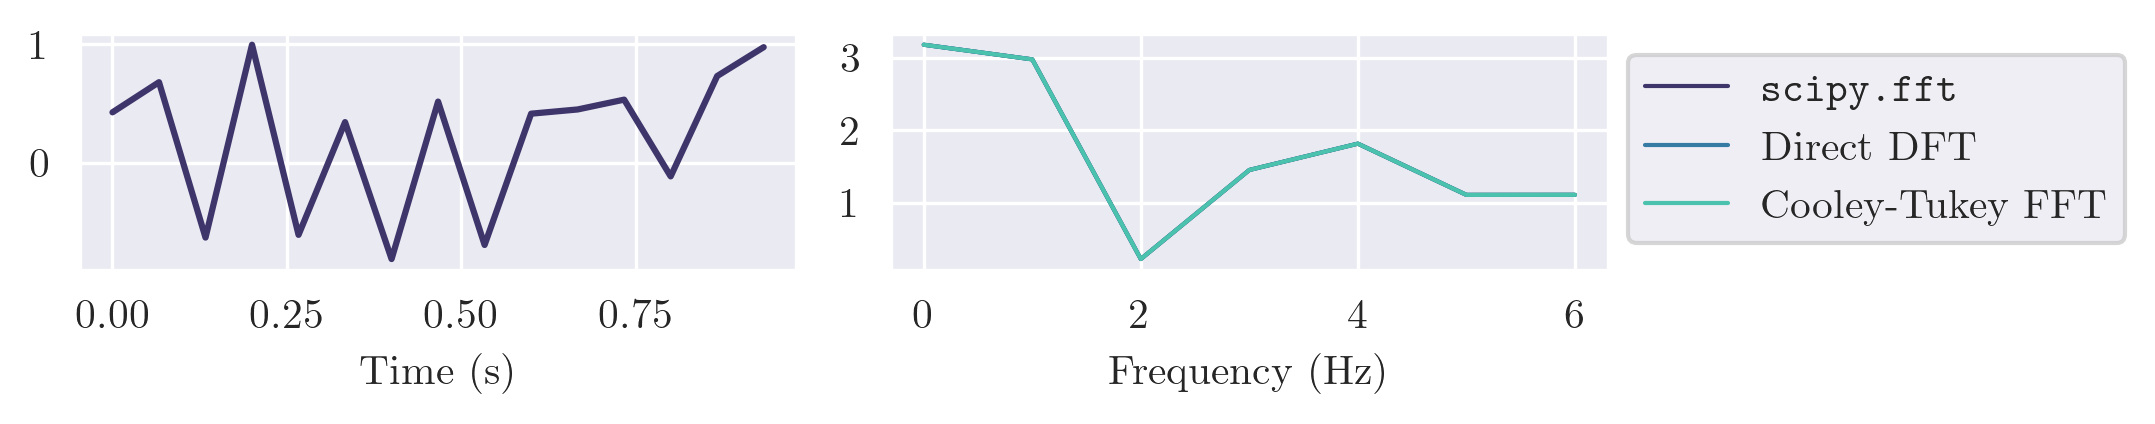
\includegraphics[width=\textwidth]{images/q6_signal.png}
    \caption{Time and frequency domain representation of a simple 15-point signal}
    \label{fig:q6_signal}
\end{figure}

\newpage

Both implementations produce the correct result and have average timings shown in Table \ref{tab:q6_timings}.

\begin{table}[ht]
    \small \centering \restretch{1.2}
    \caption{Average runtime (ms) on 15-point sequence over 10,000 trials}
    \begin{tabularx}{0.5\textwidth}{r R r}
        \toprule
        \textbf{\texttt{scipy.fft}} & \textbf{DFT} & \textbf{Cooley-Tukey FFT} \\
        \midrule
        0.007 & 0.372 & 0.246 \\
        \bottomrule
    \end{tabularx}
    \label{tab:q6_timings}
\end{table}

The Cooley-Tukey FFT demonstrates a respectable 50\% speedup over the naive DFT, even for a relatively small signal of length 15. This demonstrates the advantage of the FFT and the reason why the direct DFT is rarely used in practice. (Of course, both implementations are still dwarfed in performance by \texttt{scipy.fft}, which is no doubt optimised beyond layman sensibility.)
